\section{$c^{1}$ linearly stable flux reconstruction family of schemes}
In this section, we illustrate the process of creating a scheme that ensures $c^{1}$
flux continuity to solve the advection and advection-diffusion equation. This scheme is called C01FR, or \gls{c1fr}. We use this notation because it is possible to create a scheme whose reconstructed flux is continuous in the, say, zeroth and third derivatives without enforcing continuity in the first and second derivatives, and such scheme would have a $c^{0,3}$ flux and be called C03FR. When a scheme ensures continuity in the $0,\dots,M$ derivatives of the flux, we call it \gls{cmfr} to simplify the name, wich could as well be C012...MFR.

\subsection{C1FR for the linear advection equation}
To create the scheme with $c^{1}$ flux, we only need to find correction functions $\gL$ that satisfy \eqref{eq:gcond} and boundary conditions \eqref{eq:gconstraints}.
Let $c_0$ and $c_1$ be non-zero in Eqn. \eqref{eq:gcond}. Expanding the summation over $r$, we have the following $P+1$ equations for each $i$

\begin{equation}
\begin{split}
c_0 &\l[ \sum^S_{k=0} \theta_{ik}\l( \sum^P_{j=1}\zeta_{pj}\cdot j\cdot \ioo  \xi^{j+k-1}d\xi \r) \r] \\
&+ 
\frac{c_1}{J^2_n} \l[ \sum^S_{k=1} k \theta_{ik} \l( \sum^P_{j=2}\zeta_{pj}\cdot j\cdot (j-1)\cdot \ioo  \xi^{j+k-3}d\xi \r) \r]
 = 0
 \end{split}
\end{equation}
for $p = 1,...,P+1$.

Rearranging terms we obtain
\begin{equation}
\begin{split}
\sum^P_{j=1} \zeta_{pj} &\bigg[ \sum^S_{k=0} \theta_{ik}\bigg( c_0\cdot  j \ioo  \xi^{j+k-1}d\xi  \\
&+ \frac{c_1}{J^2_n} k j\cdot (j-1)  \ioo  \xi^{j+k-3}d\xi \bigg) \bigg]
 = 0
 \end{split}
\end{equation}

and, therefore we have the following $P$ equations, where $j = 1,\dots,P$,
\begin{equation}
\label{eqn:system}
\sum^S_{k=0} \theta_{ik}\l( c_0\cdot  j \ioo  \xi^{j+k-1}d\xi  + \frac{c_1}{J^2_n} k j\cdot (j-1)  \ioo  \xi^{j+k-3}d\xi \r) = 0
\end{equation}

We can evaluate the integral terms understanding that for positive integer $q$
\begin{equation}
\ioo \xi^q d\xi = 
\l\{
\begin{array}{ll}
\frac{2}{q+1} & \mbox{, $q$ even}\\
0 & \mbox{, $q$ odd} 
\end{array}
\r.
\end{equation}

\begin{comment}
\begin{align}
 \ioo& \l\{ \gL\xi + \frac{c_1}{J_n^2} \ddxi{\gL}(j-1)\r\}\xi^{j-2} d \xi =0 \mbox{ for }
j=1,\ldots,m\\
 \implies &\sum^s_{k=0}\theta_{ik} \ioo \l\{ \xi^{k+1} + \frac{c_1}{J_n^2} k
\xi^{k-1}(j-1)\r\}\xi^{j-2}d\xi =0
\end{align}

We want to evaluate
\begin{equation}
 \ioo \l\{ \underbrace{\xi^{k+j-1}}_{\text{\ding{172}}} + \underbrace{\frac{c_1}{J_n^2} k (j-1)
\xi^{k+j-3}}_{\text{\ding{173}}} \r\} d\xi \mbox{ , } 0\le k\le s
\end{equation}

\ding{172}:

\begin{equation}
\ioo \xi^{k+j-1} d\xi = \frac{1}{k+j} \xi^{k+j} \bigg|^1_{-1} = \frac{1}{k+j} \l[ 1-(-1)^{k+j} \r]
\end{equation}

\ding{173}:
\begin{equation}
 \frac{1}{J_n^2}\ioo c_1 k (j-1) \xi^{k+j-3} d\xi = \frac{c_1}{J_n^2} k (j-1) \frac{1}{k+j-2} \l[
1-(-1)^{k+j-2} \r] \mbox{ for
} k+j\ne2
\end{equation}
If $k+j=2$, $j=2$ and $k=0$, so
\begin{equation}
 \ioo c_1 k (j-1) \xi^{k+j-3} d\xi = 0
\end{equation}

To find the coefficients of the monomials that describe $\gL$ and $\gR$, we want to write the
constraints in matrix form:
\begin{equation}
\label{eq:gcoeff}
 0=\sum^s_{k=0} \theta_{ik} \l\{  \frac{1}{k+j} \l[1-(-1)^{k+j}\r] + \frac{c_1}{J_n^2} k
\frac{j-1}{k+j-2} \l[
1-(-1)^{k+j-2} \r] \r\} \mbox{  for  } j=1,\ldots,p
\end{equation}

Note that for $j$ odd, Eqn.~\ref{eq:gcoeff} becomes
\begin{equation}
 0 = \sum^s_{\substack{k=0\\k \text{ even}}} \theta_{ik} \l\{ \frac{2}{k+j} +2 \frac{c_1}{J_n^2} k
\frac{j-1}{k+j-2}\r\}
\end{equation}

and for $j$ even, Eqn.~\ref{eq:gcoeff} becomes
\begin{equation}
 0 = \sum^s_{\substack{k=0\\k \text{ odd}}} \theta_k \l\{ \frac{2}{k+j} +2 \frac{c_1}{J_n^2} k
\frac{j-1}{k+j-2}\r\}
\end{equation}
\end{comment}
Recalling the constraints on $\gL$,
\begin{equation}
 g^{(j)}_{L_i}(-1) = \delta_{ij} J_n^j \; ; \;   g^{(j)}_{L_i}(+1) = 0
\end{equation}

we can obtain additional equations for each $\theta_{ik}$. Specifically, for $\gL[0]$,
\begin{equation}
\begin{split}
\sum^S_{k=0} \theta_{0k}(-1)^k = 1\hspace{0.7cm} \text{ \hspace{1cm} }
&\sum^S_{k=0}
\theta_{0k}(1)^k = 0\\
\sum^S_{k=1} k\theta_{0k}(-1)^{k-1} = 0 \text{ \hspace{1cm} } &\sum^S_{k=1}
k\theta_{0k}(1)^{k-1} = 0
\end{split}
\end{equation}
and for $\gL[1]$,

\begin{equation}
\begin{split}
\sum^S_{k=0} \theta_{1k}(-1)^k = 0\hspace{0.7cm} \text{ \hspace{1cm} }
&\sum^S_{k=0}
\theta_{1k}(1)^k = 0\\
\sum^S_{k=1} k\theta_{1k}(-1)^{k-1} = J_n \text{ \hspace{1cm}} & \sum^S_{k=1}
k\theta_{1k}(1)^{k-1} = 0
\end{split}
\end{equation}

From Eqn. \eqref{eq:gr_gl_cond}, we can find $\gR$ by setting
\begin{equation}
\gR = (-1)^i\sum_{k=0}^S \theta_{ik}(-\xi)^k = \sum_{k=0}^S \theta_{ik}(-1)^{i+k}\xi^k
\end{equation}

As a result, for each $\gL$ we have $P+4$ equations. By setting $S$, the order of the correction function, to be $P+3$, we have $P+4$ unknowns and can solve a $(P+4)\times(P+4)$ system of equations to have a one-parameter, linearly stable, $c^{1}$ flux, \gls{fr} scheme.

Letting the polynomial order $P$ be $3$, we obtain the correction functions seen in Fig. \ref{fig:c1_corfunc} for varying values of $c_1$. We let $c_0 = 1$ without loss of generality (as seen by the fact that in Eqn. \eqref{eqn:system} only the ratio $c_1/c_0$ modifies the correction functions). We note that the correction functions that ensure the flux is continuous in its first derivative, namely $\gL[1]$ and $\gR[1]$ are unaffected by changes in $c_1$. On the other hand, $\gL[0]$ and $\gR[0]$ change dramatically with changes in $c_1$. In section \ref{sec:num_cases} we will see how these variations affect dispersion and dissipation properties qualitatively.

In Fig. \ref{fig:c2_corfunc} we see the correction functions corresponding to the C012FR, or C2FR, scheme with $P=3$. It is interesting to note that changes in $c_1$ affect $\gL[0]$ and $\gR[0]$ only, changes in $c_2$ affect $\gL[1]$ and $\gR[1]$ only, and $\gL[2]$ and $\gR[2]$ are not affected by $c_1$ or $c_2$.

\begin{figure}[h]
\hspace{-1.25 cm}
\centering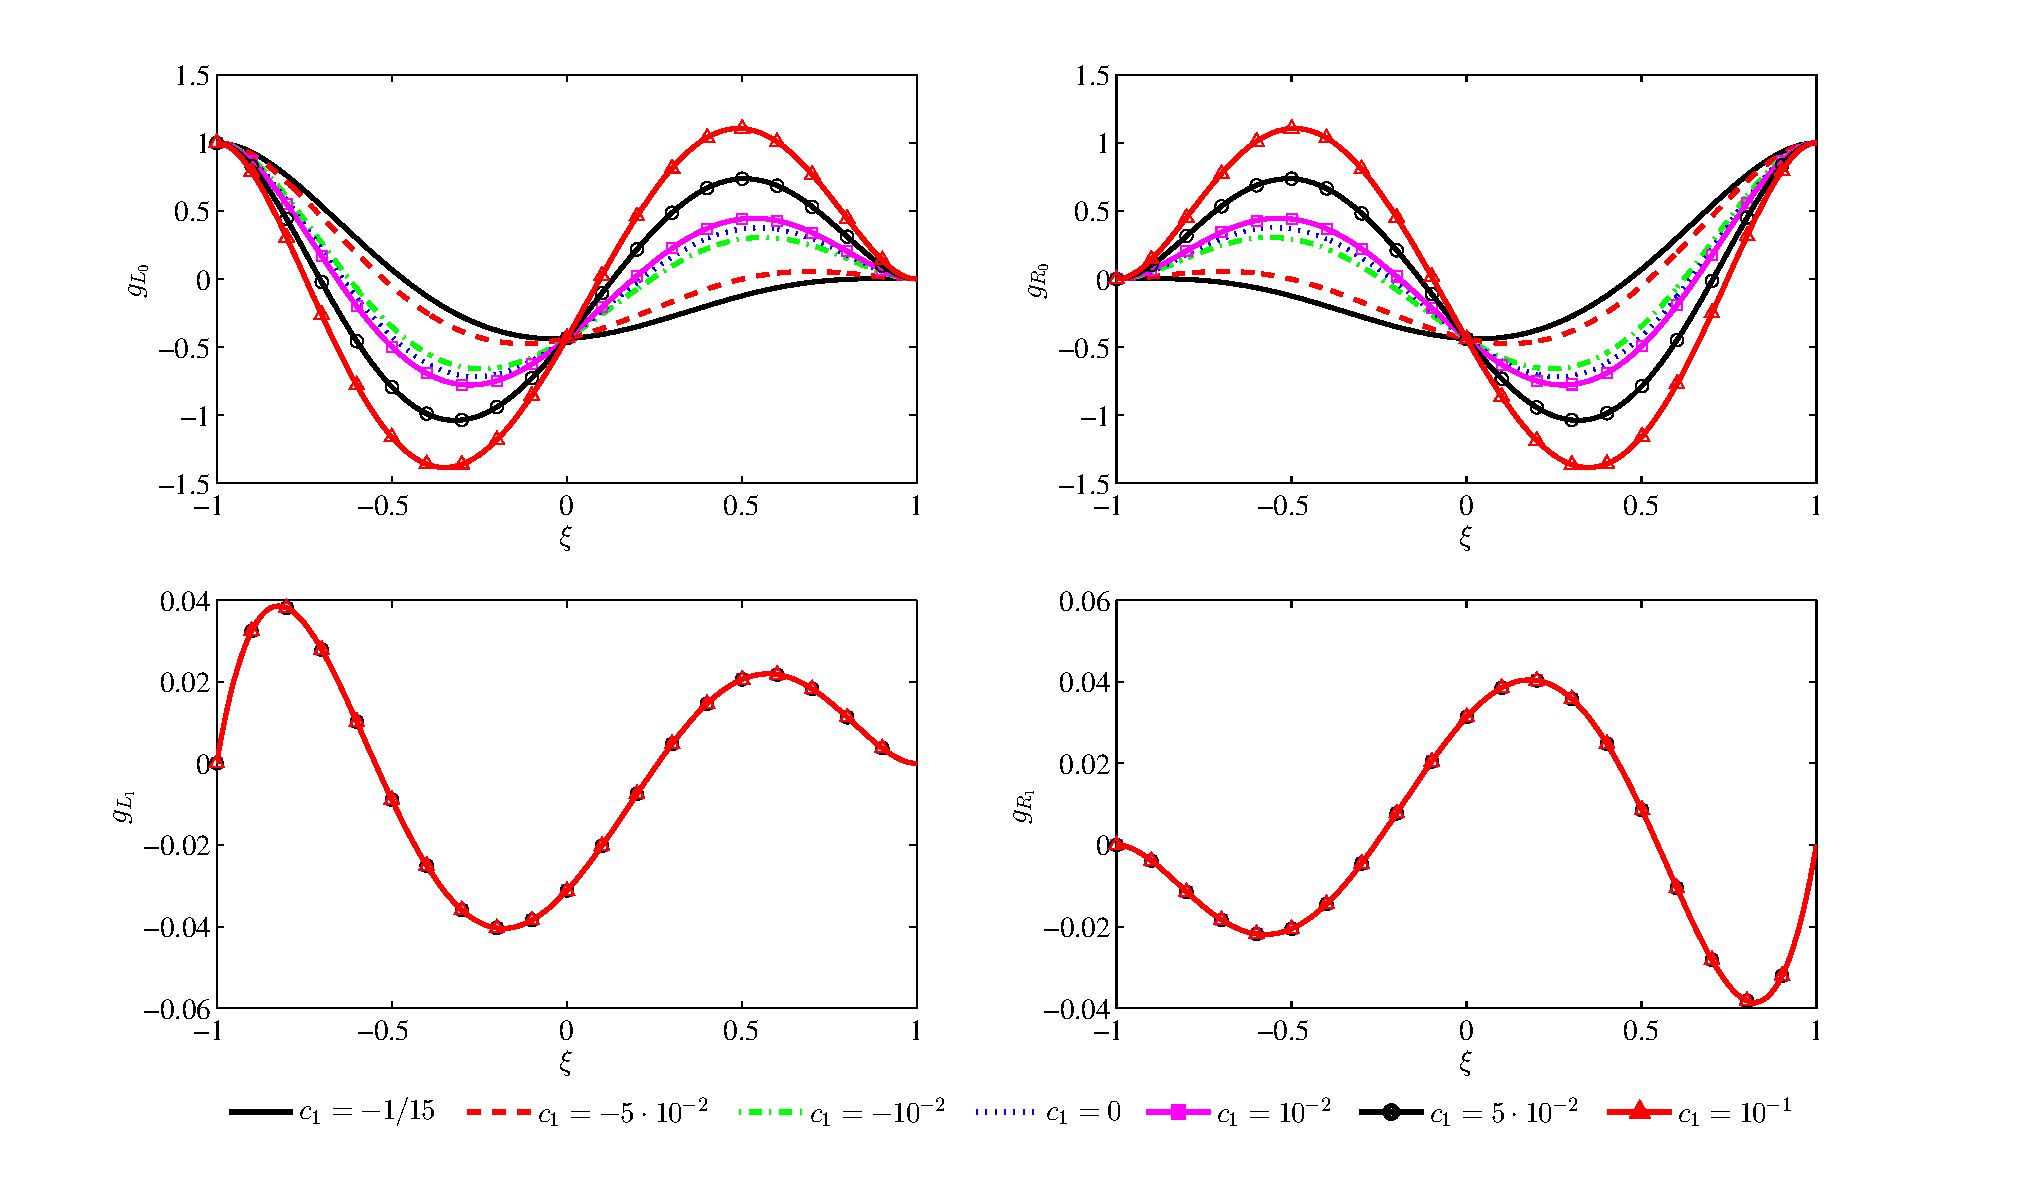
\includegraphics[width=\graphWidth\textwidth,trim=\Ltrim cm 0cm \Rtrim cm 0cm]{\cmfrdir/Figures/Correction_funcs/C1FR}
\caption{Left and right correction functions for the C1FR scheme with $P=3$, in which the zeroth and first derivatives of the corrected flux are continuous}
\label{fig:c1_corfunc}
\end{figure}

\begin{figure}[h]
\centering 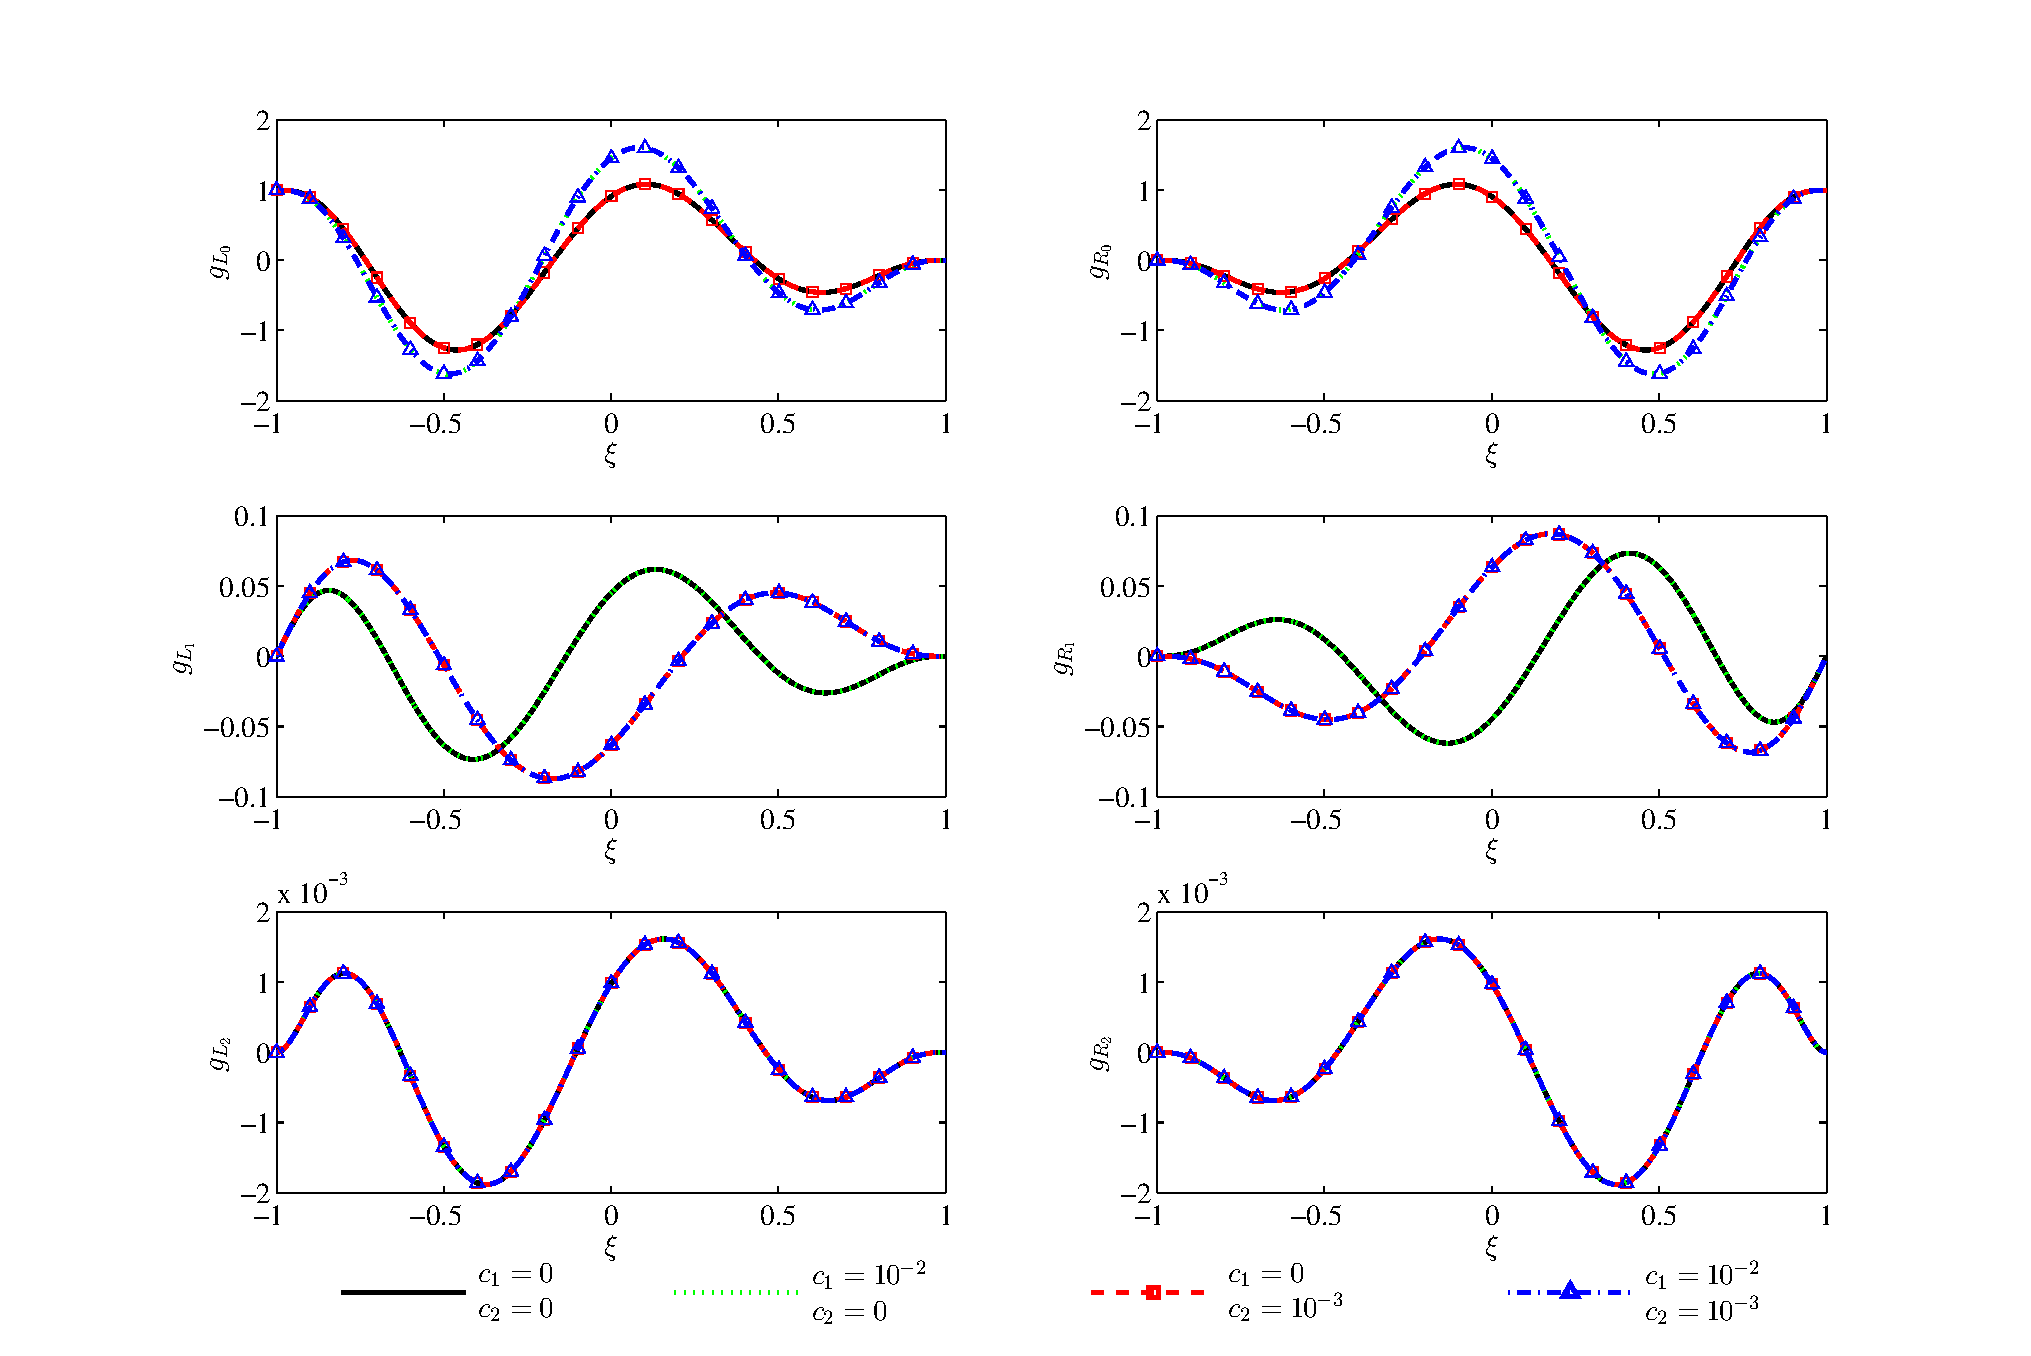
\includegraphics[width =1\textwidth,trim=\Ltrim cm 0cm \Rtrim cm 0cm]{\cmfrdir/Figures/Correction_funcs/C2FR} \caption{Left and right correction functions for the C2FR scheme with $P=3$, in which the zeroth, first, and second derivatives of the corrected flux are continuous} \label{fig:c2_corfunc} 
\end{figure}





